\documentclass{article}
\usepackage{graphicx}
% \usepackage[export]{adjustbox}
\graphicspath{ {Images/} }
\usepackage{babel}

\author{
  Dino Anastasopoulos: 1900661 \\
  Philani Mpofu: 1848751\\
  Reece James Peters: 1924514
}

\title{
  PSEUDO-KU\\
  Java Sudoku Solver using Backtracking
}

\date{07 October 2020}

\begin{document}
    \begin{titlepage}
        \maketitle{}
    \end{titlepage}
    
    \tableofcontents

    % Aims
    \pagebreak 
    \section{Aims}
    The main aim of this lab report is to review the performance of our group’s implementation of the Backtracking Algorithm on solving sudoku puzzles with varying amounts of incomplete cells (having value 0). Conversely, one could also interpret it as reviewing the algorithm’s performance on solving sudoku puzzles with varying amounts of completed cells or clues (having non zero values). In this report, we hypothesize that puzzles with fewer clues (more cells with 0 values) will require more computation in order to be solved.


    It is thus our goal to verify our theoretical assumptions (which will be expanded upon in subsequent sections) of the algorithm’s performance with the empirical evidence we obtain from testing our algorithm on many different sudoku puzzles. Simply put, we want to check that the algorithm has the same space and time complexities that we believe it to have theoretically. If this is not the case, then it is also our goal to determine why it is not. 


    % Summary of Theory
    % \pagebreak 
    \section{Summary of Theory}
    Our initial assumption is that the Backtracking Algorithm will have the following space and time complexities when solving 9x9 sudoku puzzles:


    \subsection{Space Complexity : O($n^2$)}
    The initial and solved sudoku puzzle would need to be stored in a 2D matrix made up arrays of size n. Thus, in any case the space complexity would be O($n^2$). \cite{GeeksforGeeks}


    \subsection{Time complexity: O$(9^{n^2})$} 
    There exists 9 possible options for every incomplete cell. In the worst case, the algorithm would need to visit every incomplete cell in every iteration and change all of the values 9 times. Thus, the time complexity in this case would be O$(9^{n^2})$ where n is the number of incomplete cells. In the best case, the algorithm would need to visit every incomplete cell once and change the value once only. Thus, the time complexity in the best case would be O($n^2$). \cite{GeeksforGeeks}
    

    % Experimental Methodology
    \pagebreak 
    \section{Experimental Methodology}
    As stated in our aims, our initial assumption is that puzzles with more incomplete cells (or fewer clues) will result in more computation needed to find the unique solution. We have utilized 4 metrics to measure the performance of the algorithm, namely the number of comparisons, number of changes, number of recursive calls, and the amount of time taken to return a unique solution to a given puzzle. Please see below discussions on our chosen metrics:

    \subsection{Number of comparisons}
    This metric measures the number of times the program compares the value chosen for a current cell with another value on the board. The value is compared against every other value in the chosen cell's row, column, and 3-by-3 sub-grid, in order to determine if it safe to place in the cell.

    \subsection{Number of changes}
    This metric measures the number of times the program determines that a specific value is safe to enter in the current cell and so changes its value from a zero (incomplete cell), to the determined number, or from a previosuly determined number to another "safe" number.
    
    \subsection{Number of Recursive Calls}
    This metric measures the number of times the program is recursively called to find a unique solution to the given puzzle. Whenever the program finds a value that is "safe" for a specific cell it updates the board and then calls the function again until the algorithm gets to a cell that has no "safe" value - at which point it will backtrack, change the number of a previosuly determined cell, and start recursevely calling the function again.

    \subsection{Run Time}   
    This metric measures the length of time (in milliseconds) it takes for the program to solve a given puzzle. 


    It is our assumption that puzzles with more incomplete cells will need more comparisons, more changes, more recursive calls and a longer runtime than puzzles with less incomplete cells(more clues).\cite{{inproceedings}}

    \pagebreak
    Initially, we had decided to use a puzzle’s difficulty (easy, medium, difficult, expert) as the independent variable to measure the performance of our algorithm. We had plotted the difficulty of the graph against the number of comparisons, changes, recursive calls and run time to solve the puzzle. However, this metric was abandoned for a number of reasons. 
    Firstly, the graphs that were generated using this variable gave very little insight to the performance of our program (if any). This was due to the fact that easy puzzles generally have 38 clues, and expert puzzles have up to 21 clues at a minimum, which is not a big enough range to accurately measure the performance.
    Secondly, we found that in some cases puzzles of varying difficulties gave the same results. This is obviously incorrect, because an easy puzzle should not be getting the same results as a medium puzzle for example. We discovered that a "difficult" easy puzzle would yield the same results as an "easy" medium puzzle. 
    Thirdly, it is very difficult to define a puzzle’s difficulty by a word rather than a scale of values as it is a concept that can be understood by a human, but it would be very abstract to a computer. 
    
    
    We then realized it would be a better option to analyse our algorithm based on number of clues as a way to determine that puzzle’s difficulty.  
    To measure the performance of our program we started off with the initial solved puzzle, ran our program on it and recorded and plotted the results. Then we randomly removed 1 clue at time from that puzzle and tested the algorithm on it. This process was repeated until there were no more clues left in that puzzle (ie: the puzzle was left only with incomplete cells). We repeated this on multiple boards and averaged the results to get a more general set of results. This process made up our empirical experimentation. Below are some illustrations of a few of the iterations of the algorithm performed on puzzle taken from Sudoku.com \cite{{Sudoku:2020}}


    \begin{figure}[!htb]
    \minipage{0.32\textwidth}
      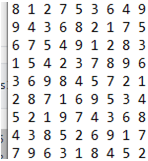
\includegraphics[width=\linewidth]{iteration1.png}
      \caption{Iteration 0}\label{fig:awesome_image1}
    \endminipage\hfill
    \minipage{0.32\textwidth}
      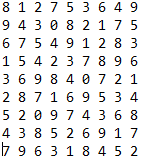
\includegraphics[width=\linewidth]{iteration2.png}
      \caption{Iteration 3}\label{fig:awesome_image2}
    \endminipage\hfill
    \minipage{0.32\textwidth}%
      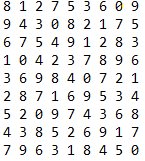
\includegraphics[width=\linewidth]{iteration3.png}
      \caption{Iteration 6}\label{fig:awesome_image3}
    \endminipage
    \end{figure}


    As you can see, the puzzle in the first iteration has no white spaces since it is the solved puzzle. The puzzle in the third iteration has white spaces in positions (1,3), (4, 5) and (6,3). The puzzle in the sixth iteration has white spaces in positions (1,3), (4,5), (6,3), (0,7), (3,1) and (8,8). Results of the performance of this implementation of the algorithm will be presented, interpreted and reviewed in subsequent sections.
     
    % Presentation of results
    \pagebreak 
    \section{Presentation of results}
    \begin{figure}[h]t
        \centering
        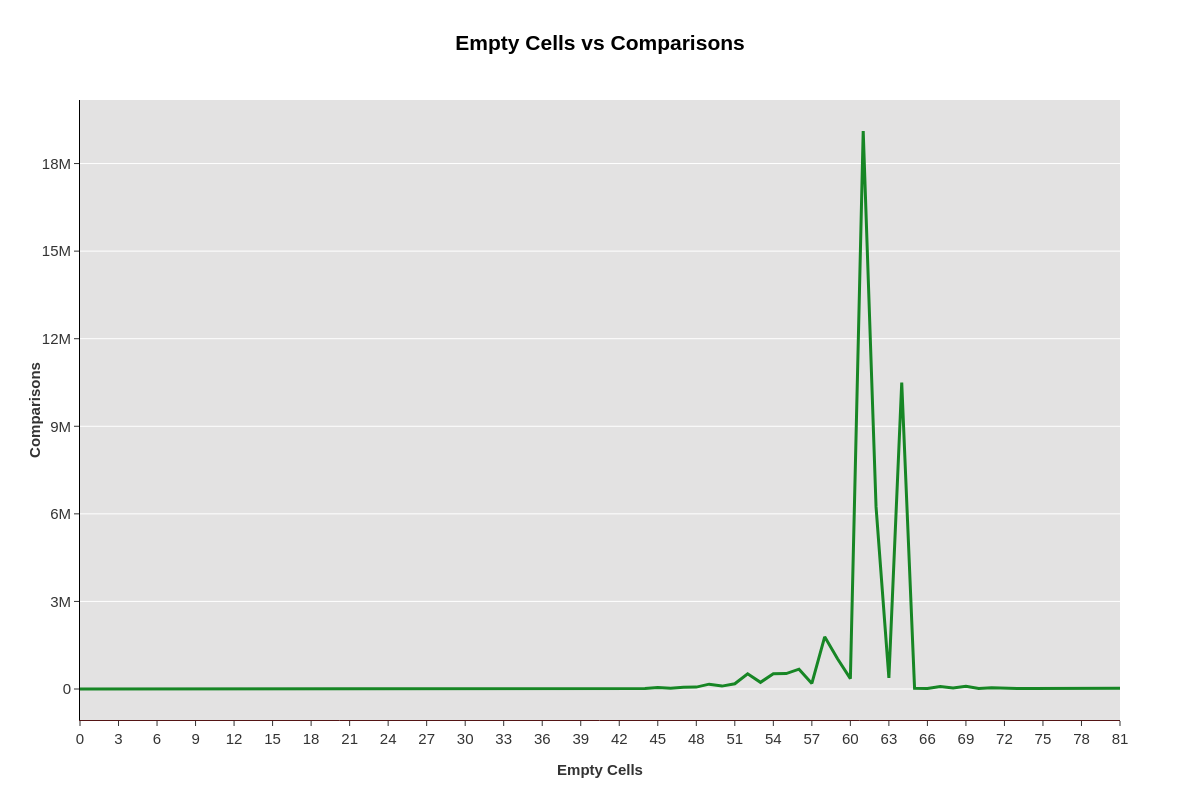
\includegraphics[width=0.75\textwidth]{Comparisons.png}
        \caption{Number of Comparisons}
    \end{figure}
    
        \begin{figure}[ht]
        \centering
        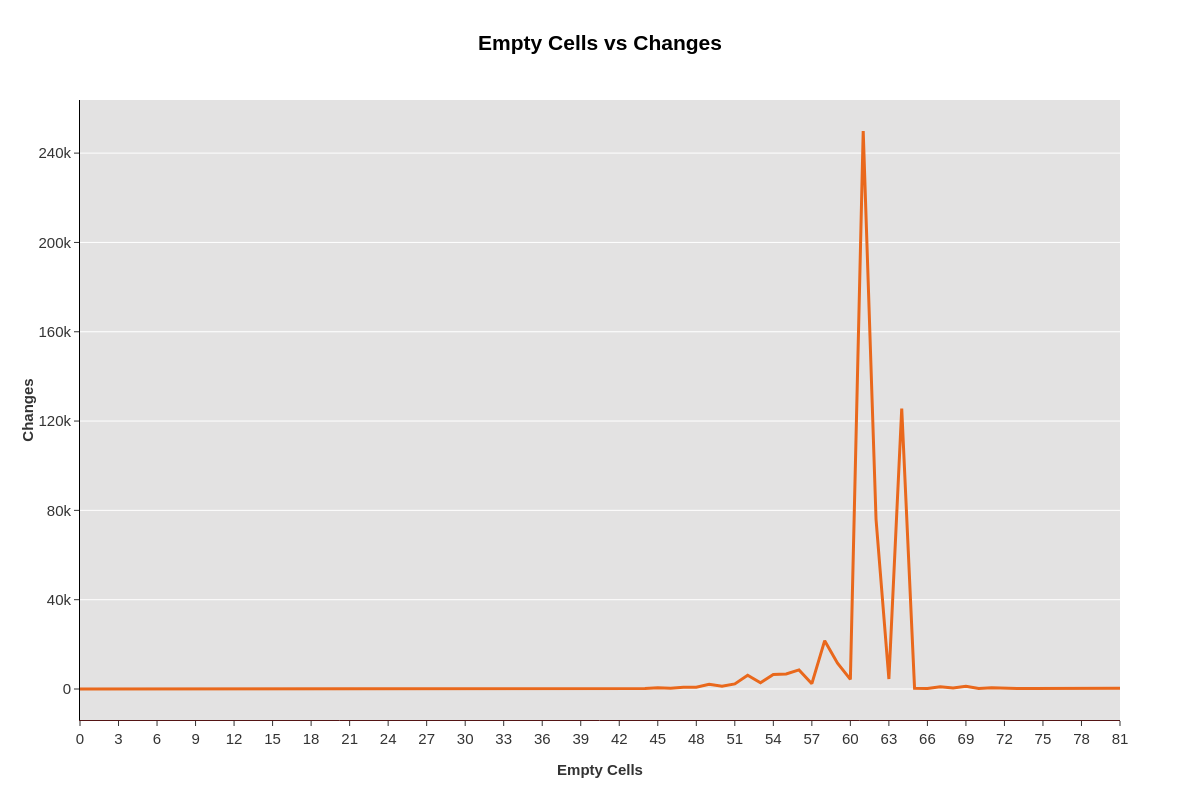
\includegraphics[width=0.75\textwidth]{Changes.png}
        \caption{Number of Changes}
    \end{figure}
    
        \begin{figure}[ht]
        \centering
        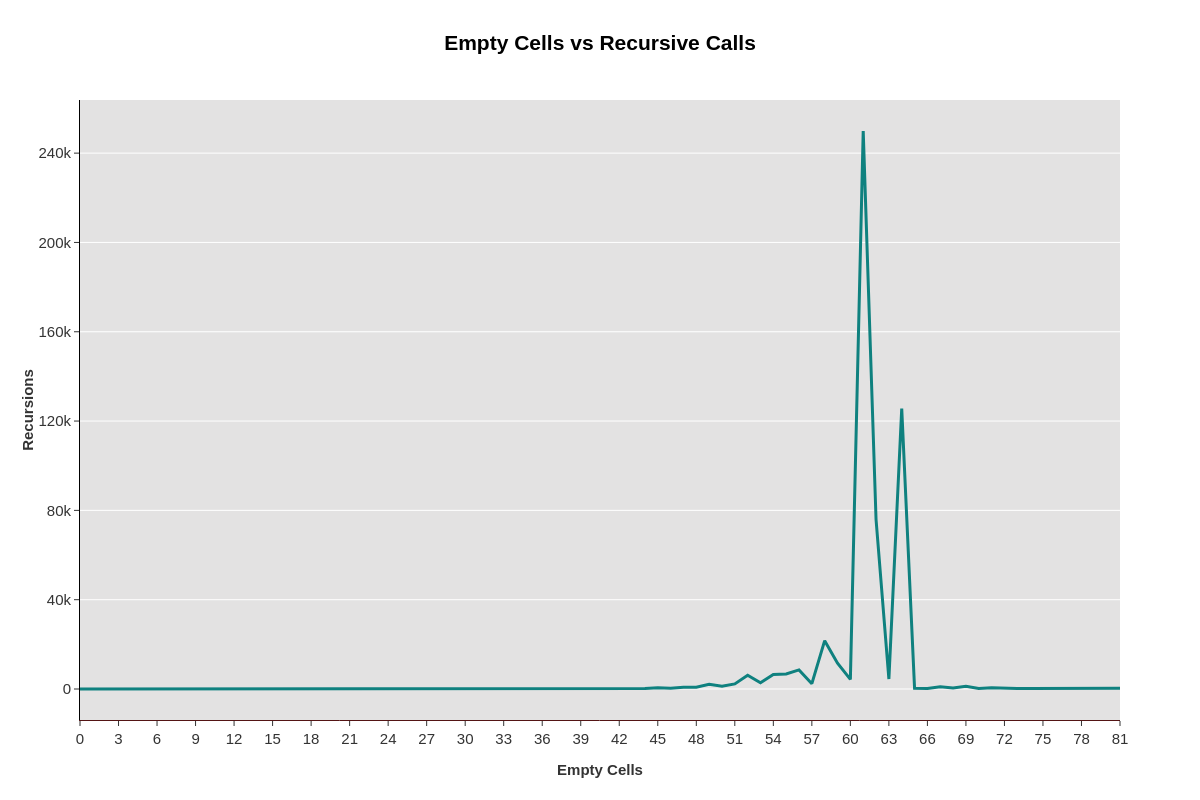
\includegraphics[width=0.75\textwidth]{Recursions.png}
        \caption{Number of Recursive Calls}
    \end{figure}
    
        \begin{figure}[ht]
        \centering
        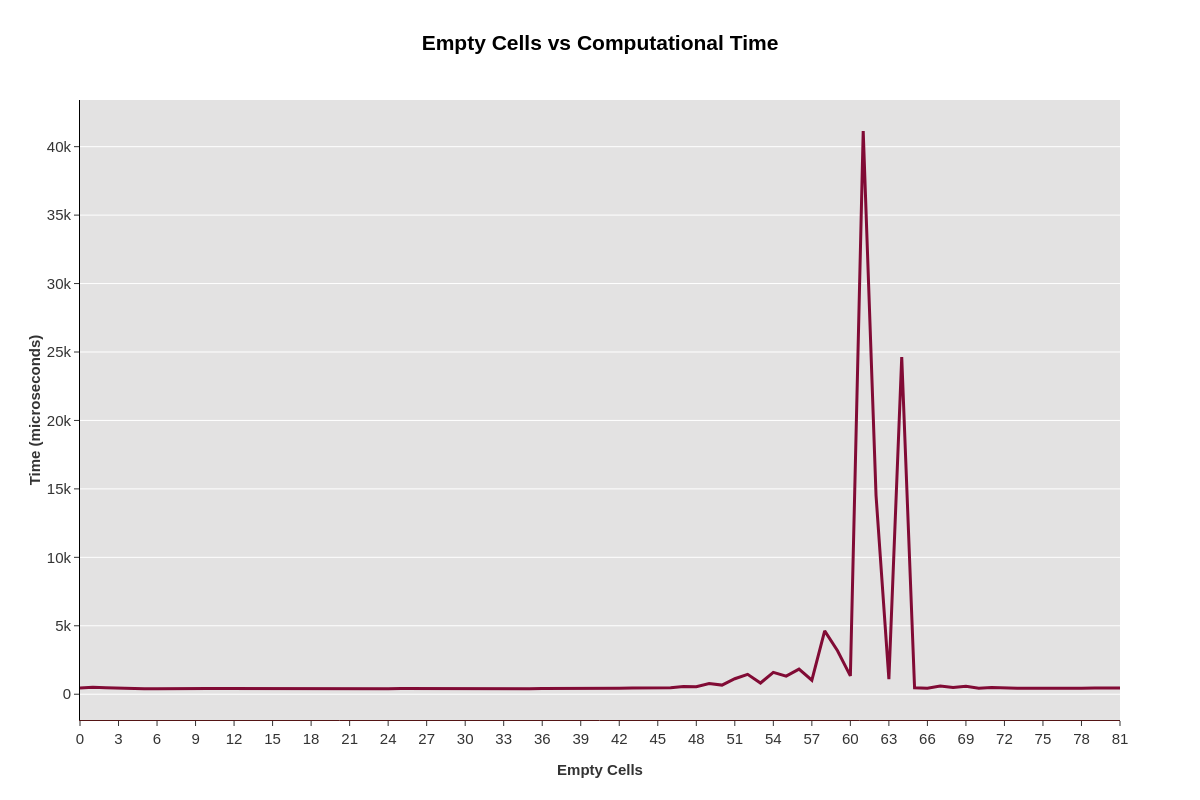
\includegraphics[width=0.75\textwidth]{Time.png}
        \caption{Run Time}
    \end{figure}


	\clearpage
    % Interpretation of results
    \pagebreak
    \section{Interpretation of results}
    The results obtained, while occasionally inconsistent, did lend to the discovery of trends and patterns within the performance of the algorithm. All four metrics grew, and shrunk, at incredibly similar rates. This makes sense since changes to a cell can only be made once it has been compared to other cells, and time is directly tied to the number of processes that need to run (i.e. array accesses, integer comparisons, and variable changes). 
        

    During the very early iterations (0-20 incomplete cells) the metrics were quite similar, in that they were fairly low and did not seem to grow a significant amount as clues were removed. This is most probably due to the fact that the algorithm was finding the correct number for each incomplete cell on its first or second try, as there was abundance of clues on the board deterring the algorithm from placing the wrong number in each cell. 
    
 
    As the number of incomplete cells grew beyond this point (20-40 incomplete cells) the metrics began to grow slightly faster, but still quite linearly. We assume this is tied to the reasoning in the previous paragraph, and growth can attributed to the fact that more cells were incomplete at each iteration, so while the algorithm was still finding the solution for each cell rather quickly, there were simply more cells to check and fill.


    It should be noted that time was fairly constant for all aforementioned states. This is most likely due to the fact that the minuscule increases in comparisons and changes made little to no difference to the processing capacity of our 21st century computers.


    The meat of the growth lies in this next interval (40-60 incomplete cells). The increase in all metrics was exponential and usually maxed out between 55 and 65 incomplete cells). We assume this is due to the fact that at this point the board starts having more incomplete cells than clues. This means the algorithm has more cells to fill and less information to guide it to the correct answer. As such it will naturally go through more and more recursions to find the correct value for each cell, as it is unlikely to find them early on. Thus, more comparisons will be made for each cell as well. These factors compound to give us the exponential growth observed. It is also, unsurprisingly, in this interval that the time complexity starts increasing.


    A very unexpected discovery is what happens during the last interval (60-81 incomplete cells). All metrics seem to drop rapidly and then stay fairly consistent until the end. We have deduced that this is due to the fact that there are so few clues left on the board that the algorithm has very few restrictions on which value it is allowed to place in each cell, and thus finds the result fairly quickly as there are numerous solutions that can be built from the very few number of clues. At this point the algorithm is basically making its own solution to the puzzle. 

    % Theory relationship
    \pagebreak 
    \section{Theory relationship}
    The results have both confirmed and debunked our theories. We expected to see constant exponential growth due to the factors we had anticipated throughout the data, but this was only the case for the interval of 40-60 incomplete cells. The rest of the datapoints were fairly similar and linear due to the nature of sudoku and the approach our algorithm takes to solve it.


    It is interesting to note that that sudoku generally measures its difficulty on its number of clues, where easy puzzles tend to have about 38 clues (43 incomplete cells), medium puzzles about 30 clues (51 incomplete cells) and difficult ones about 22 clues (59 incomplete cells). It is no coincidence that all of these lie within the interval where we noticed most of our expected trends. Anything less or more and the puzzle simply becomes too easy for both human and computer alike. 

    % Conclusion
    % \pagebreak 
    \section{Conclusion}
    It has been determined that our algorithm does have a complexity of O$(9^{n^2})$ but only when the data lies within a certain interval. The best case runs in O($n^2$) and occurs when all incomplete cells are the only incomplete cell in their row, column and sub grid which results in only 1 "legal" value that can be chosen. The worst case runs in O$(9^{n^2})$ and occurs when there are about twice as many incomplete cells as there are clues. Due to the strange nature of the data and sudoku as a whole, the ‘average’ case does not seem to be determinate.

    % References
    \pagebreak
   % \section{References}
    \bibliographystyle{plain}
    \bibliography{file.bib}

    % Acknowledgements
    % \pagebreak 
\end{document}
